
We calculate \rev{gyrochronological ages} using the python package \texttt{gyro-interp} which computes age posteriors by interpolating between rotation sequence models for open clusters with well-defined ages \citep{2023ApJ...947L...3B}. \texttt{gyro-interp} is calibrated for stars with $3800 K < T_{eff} < 6200 K$. We measure rotation periods from $TESS$ light curves processed with the SPOC pipeline \citep{2016SPIE.9913E..3EJ}, which were available for 129 of our target stars. We visually inspect each light curve and its corresponding Lomb-Scargle periodogram \citep{1976Ap&SS..39..447L, 1982ApJ...263..835S} to make an initial estimate for the rotation period. \rev{Then, to further validate and refine the selected period}, we use the non-linear least squares fitting python package \textit{LMFIT} \citep{2016ascl.soft06014N} to fit a sinusoid to the light curve. We run \textit{LMFIT} to find the sinusoid's amplitude, phase, vertical offset, and period. We limit the period to a narrow range around the initial estimate to prevent the fit from getting stuck at a local minimum at a harmonic of the true period. \rev{We do not use MCMC or another sampling algorithm to find the rotation period because a sinusoid is only an approximation of spot modulation and because photometric measurements are correlated over small time spans.} 

To ensure we select an actual rotation signal we compare our adopted period to peaks in the corrected (PDCSAP) and the uncorrected (SAP) periodograms. The period must appear as a local maximum in both periodograms to be accepted. We do not require the period to be the global maximum of either periodogram.

We differentiate between ``flat" light curves and robust variability signals by comparing $\chi^{2}$ for a flat line and the best-fitting sinusoid. Based on visual inspection of light curves from our target stars, we identify light curves with $\Delta \chi^{2} \gtrsim500$ as having a variability signal, and classify all other light curves as flat. Regardless of their $\Delta  \chi^{2}$, \rev{25} stars have variability amplitudes $\lesssim0.1\%$ and are taken to be flat. We also visually confirm variability in each light curve. We do not measure rotation periods for 8 stars that share a $TESS$ pixel with another star that is $\gtrsim2.5\%$ as bright as the target star in the \textit{Gaia} G band. We also visually inspect the target-pixel files (TPFs) for bright stars on the edges of nearby pixels.

For stars observed in multiple $TESS$ sectors, we adopt the period from the \rev{light curve with the fewest and/or smallest down-link gaps, which we determine by visual inspection. If more than one curve has similar amounts of data gaps, we select the light curve with the highest signal-to-noise.} We use the other sectors to further validate our adopted rotation periods. Some stars are not variable in some sectors but are highly variable in others. We attribute this to spot evolution, such that spots are present in one sector but not present in another. We adopt the rotation period from the sector displaying variability.

\rev{Measuring rotation period uncertainties can be challenging, and there are several different methods commonly used. For example, \cite{2021AJ....162..147H, 2019ApJS..244...21S, 2021ApJS..255...17S} estimate rotation uncertainties by the width of the periodogram peak, while \cite{2020ApJ...903...99H} use the width of the autocorrelation peak. We estimate uncertainties on the measured rotation periods with a similar method, by fitting a Gaussian to the exponentiated Lomb-Scargle periodogram peak, which is proportional to the likelihood of a single-sinusoid model at each frequency \citep{2018ApJS..236...16V, 2020sdmm.book.....I}. \cite{2018ApJS..236...16V} cautions that this method does not take into account the possibility of having selected the wrong periodogram peak. Therefore, we validate our period selection in two ways: visual inspection and false alarm probability (FAP). For all our measured periods, the largest FAP we calculate is $0.5\%$, and all the light curves cover more than one period making visual identification of the period relatively robust. We propagate the $\sigma$ of the best fitting Gaussian in frequency space to period, such that
\begin{equation}
    \sigma_{P} = \sigma_{f}P^{2}
\end{equation}}


%We estimate uncertainties on the measured rotation periods by visually inspecting how well sinusoids with the adopted period adjusted by 2.5, 5, 10, 15, and 20$\%$ trace the light curve as shown in Figure \ref{gyro-TESS}. The largest change in period that is still consistent with the full sector’s light curve, based on visual inspection, is taken as the error on the period. 

We use \texttt{gyro-interp} \citep{2023ApJ...947L...3B} to turn these rotation periods and uncertainties into age posteriors, with an example \rev{gyrochronological age} posterior shown in Figure \ref{gyro-post}. \rev{\texttt{gyro-interp} generates age posteriors from rotational periods in a similar manner to how \texttt{BAFFLES} generates posteriors from lithium and calcium measurements. A reference sample of stars in clusters and associations of known ages was used to find the distribution in rotation period as a function of age and temperature, as well as the astrophysical scatter. The generated age posterior is then a combination of the rotation period and errors and the astrophysical scatter. As with lithium, the dominant source of uncertainty in the final posterior is astrophysical scatter rather than measurement uncertainty on the period.}


\begin{figure*}[ht!]
\centering
 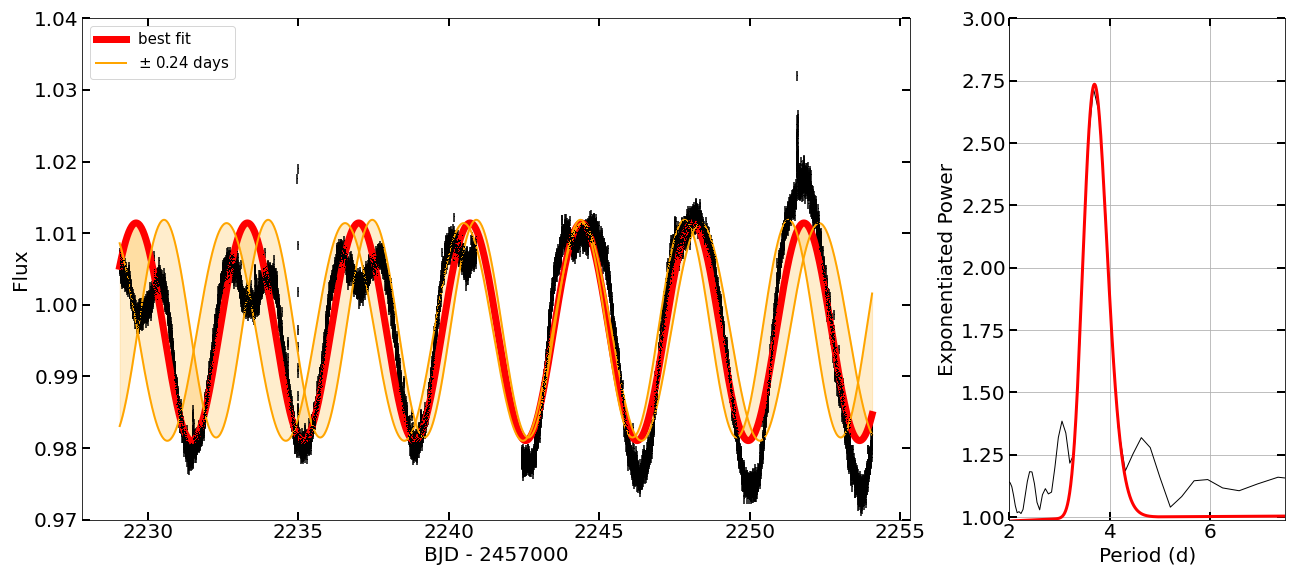
\includegraphics[scale = 0.35]{exampleLC.png}

 \caption{\rev{We measure rotation periods for the accelerating stars by analyzing their periodograms and fitting sinusoids to their lightcurves. The $TESS$ light curve for HIP 41277 is shown in black with the best fitting sinusoid with a period of 3.7 days overplotted in red. The orange curves represent the best-fitting period adjusted by the uncertainty measured from the width of the exponentiated periodogram peak. The right-hand panel shows the exponentiated Lomb-Scargle periodogram with a significant peak at $\sim3.7$ days and the best fitting Gaussian.}}
 \label{gyro-TESS}
\end{figure*}


\begin{figure*}[ht!]
\centering
 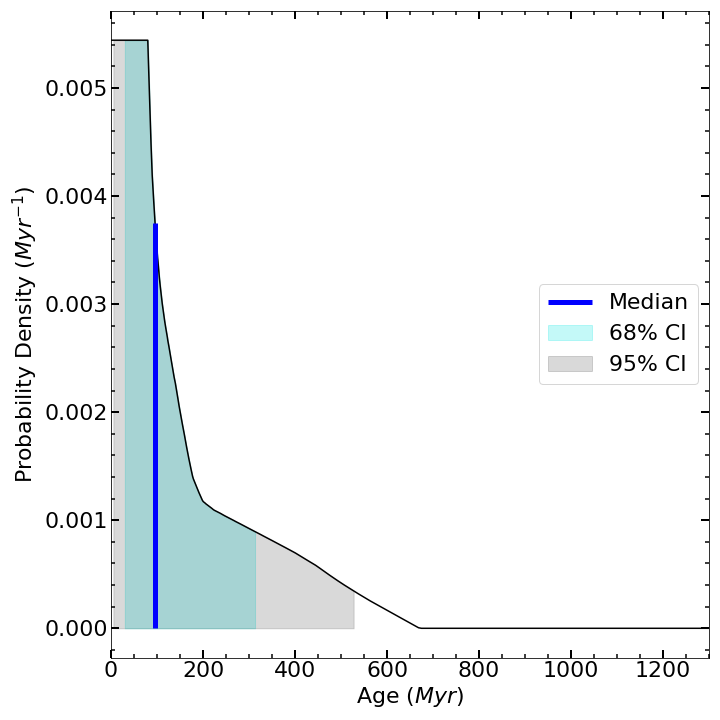
\includegraphics[scale = 0.375]{example_gyro_post.png}

 \caption{We calculate age posteriors from rotation periods using \texttt{gyro-interp} \citep{2023ApJ...947L...3B}. The age posterior for HIP 41277 with an adopted $T_{eff}$ of $4551\pm195$K and a measured rotation period of $3.70\pm0.24$ days has a median age of 96 Myr and a $68\%$ confidence interval between 30 and 316 Myr.}
 \label{gyro-post}
\end{figure*}


\subsection{Complex light curves}

Several $TESS$ light curves of our targets do not exhibit straightforward rotation signals. In this section, we briefly describe the different types of variability we observe \rev{(e.g. \citealt{2013MNRAS.432.1203M}).}

{\bf Double periods - } HIP 117410 shows two distinct periods in its light curves, but is not on obviously contaminated pixels. We interpret this as a rotation signal of two stars on the same pixels. To determine each period, we visually assess each light curve and make an initial estimate for each period. Then, we fit a double sinusoid to the flux of the form, 
\begin{equation}
    F = A_{1}\sin(2\pi f_{1} t + \phi_{1}) +  A_{2}\sin(2\pi f_{2} t + \phi_{2})
\end{equation}
 to each light curve using \textit{LMFIT}. $f_{1}$ and $f_{2}$ are the frequencies, $A_{1}$ and $A_{2}$ are the amplitudes, and $\phi_{1}$ and $\phi_{2}$ are the phase shifts of each of the component sinusoids. We find the best fitting periods for each component to be $10.65\pm1.07$ days and $0.69\pm0.07$ days. The best-fitting double sinusoid for HIP 117410 is shown in Figure \ref{2_periods}. 
 
 HIP 117410 (WDS 23484-1259) is a $\sim1"$ double star with a flux ratio of $\sim4$ in $V$ band \citep{2001AJ....122.3466M}, so this pair is most likely the source of the two signals. This pair was not flagged as a contaminated pixel due to the absence of a \textit{Gaia} G band measurement for the secondary. Early analysis of the APO/ARCES radial velocities of HIP 117410 (to be discussed in detail in a future paper) suggests that the system is not a short-period stellar binary.
 
 We cannot determine which period corresponds to which star, or directly measure $B-V$ for the secondary with the current data. Instead, we derive an age posterior for each period with the B-V of the primary, then marginalize over each star by summing the two posteriors and normalizing the resulting posterior so that it integrates to 1 (Table \ref{table:117410}). 


 \begin{figure*}[ht!]
\centering
 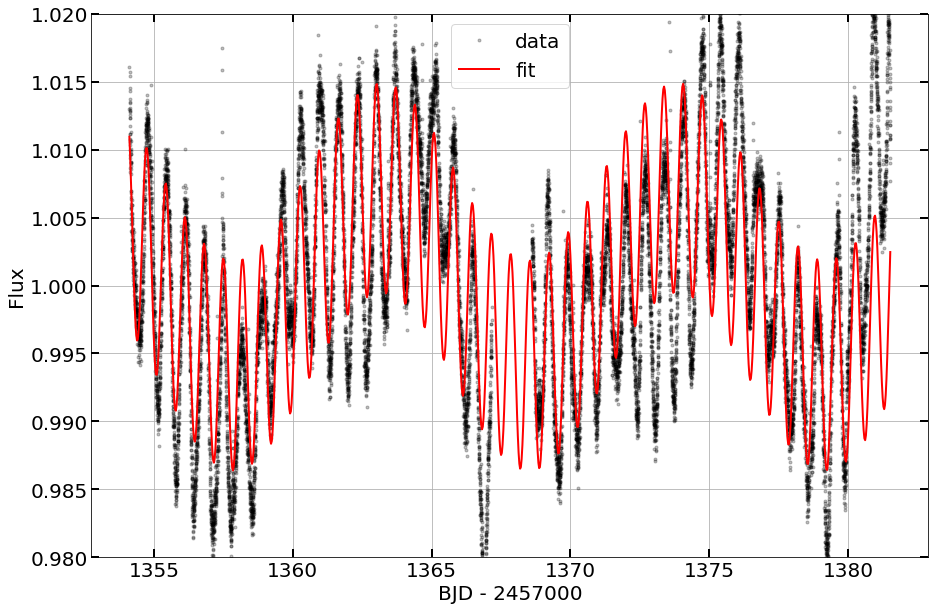
\includegraphics[scale = 0.3]{double_sine_for_paper.png}

 \caption{We fit a two-component sinusoid model (red) to a light curve (black) for HIP 117410. We find the periods of the two components to be $10.65\pm1.07$ days and $0.69\pm0.07$ days}
 \label{2_periods}
\end{figure*}





\begin{table}[ht!]
\centering

 \begin{tabular}{|c|c|c|c|}
   
     
     \hline
        $ P_{rot}$ & Age & $68\%$ CI & $95\%$ CI \\
          (d) & (Myr) & (Myr) & (Myr)  \\
       \hline

      $10.65\pm1.07$ & 415.99  & 214.20--967.37  & 146.59--11492.34\\
      
       $0.69\pm0.07$ & 105.19 & 32.77--337.67 & 5.56--542.49 \\
      
      Combined & 254.07 & 64.24--625.41 & 10.11--1400.23 \\
      
     \hline

     
      
   
\end{tabular}

     

\caption{The age posteriors for HIP 117410 for both periods and the combined posteriors are listed. We adopt the combined age posterior for this system.}

\label{table:117410}
\end{table}

{\bf Eclipsing Binaries - }\rev{We identify HIP 16247, HIP 45731, and HIP 49577 as eclipsing binaries. HIP 45731 and HIP 16247 were previously analyzed in \cite{2022ApJS..258...16P} and \cite{2023A&A...672A.119G}, respectively.}

We calculate the orbital period and rotational periods separately for each of these three systems. To find the orbital period we phase-fold the light curve based on the highest periodogram peak, verifying that the eclipses overlap, and the primary and secondary eclipses are not repeated in the folded light curve. If the phase folded curve has too many eclipses or the eclipses do not overlap, we try the next harmonic. We estimate the uncertainty of the orbital period by altering the period until the eclipses no longer overlap in the phase-folded light curve. To measure the underlying rotational period, we mask out the eclipses and then use the method described above for single stars. Table \ref{table:EBS} gives the orbital periods ($P_{o}$) and rotational periods ($P_{r}$) for each system as well as approximate depths of the primary ($D_{p}$) and secondary ($D_{s}$) eclipses. Figure \ref{EB_ex} shows the light curve for the eclipsing binary HIP 16247 with the best fitting sinusoid to the underlying rotation plotted in red. \rev{The data and the sinusoid fit are out of phase with each other between $1420 < BJD - 2457000 < 1425$. We attribute this to the fact that a simple sinusoid does not account for spot evolution and changing amplitudes, which can shift the phase of the periodicity, but a sinusoid is sufficient for capturing the periodicity of the underlying rotation rate.}

\begin{figure*}[ht!]
\centering
 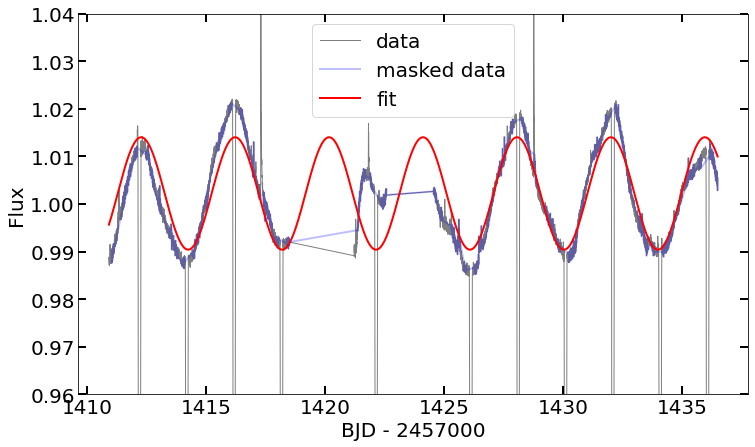
\includegraphics[scale = 0.35]{EB_rotation-1.png}

 \caption{We fit a sinusoid to the underlying rotation signal of an eclipsing binary system. The light curve for HIP 16247 is shown in gray. The masked data with the eclipses removed is shown in purple, and the best-fitting sinusoid is shown in red. This star is tidally locked with $P_{orb} \approx P_{rot} \approx 3.98$ days.}
 \label{EB_ex}
\end{figure*}




\begin{table}[ht!]
\centering

 \begin{tabular}{|c|c|c|c|c|c|}
   
     
     \hline
      Target & WDS & $ P_{o}$ & $D_{p}$ & $D_{s}$ & $P_{r}$\\
            & &(d) & & & (d)  \\
       \hline
    
      HIP 16247 & 03294-2406 &  $3.98\pm0.004$ &  $\sim28\%$ &  $\sim22\%$ & $3.95\pm0.4$ \\
 
      HIP 45731 & 09194+6203&  $2.92\pm0.003$&  $\sim15\%$ &  $\sim14\%$ & $2.92\pm0.3$ \\
  
      HIP 49577 & -- &  $16.85\pm0.17$ &  $\sim24\%$ &  $\sim10\%$ & $7.2\pm0.72$ \\
     \hline

    
   
\end{tabular}

     

\caption{The estimated parameters of the three eclipsing binaries in our sample.}
\label{table:EBS}
\end{table}
\begin{figure*}[hb!]
\centering
 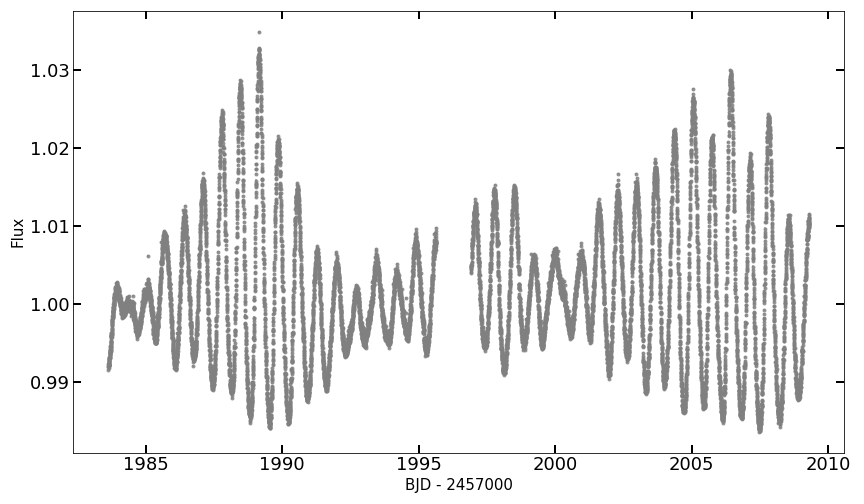
\includegraphics[scale = 0.3]{exampleLC_beat.png}

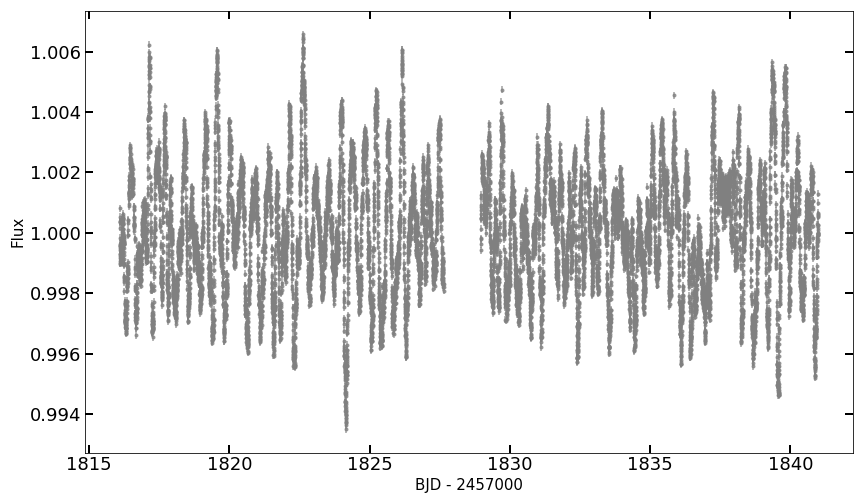
\includegraphics[scale = 0.3]{exampleLC_stochastic.png}
 \caption{Several of our target stars exhibit photometric variability that is inconsistent with rotation. {\bf Top:} A light curve of HIP 59767, a $\gamma$ Doradus variable \citep{2016MNRAS.458.2307K}, shows a beat pattern making it difficult to measure an underlying rotation period. {\bf Bottom:} A light curve of HIP 22361 shows stochastic variability that is not attributed to rotation.}
 
 \label{notrot_ex}
\end{figure*}

In close binaries, the stars can be spun up by tidal forces, so that the rotation period reflects tidal evolution rather than spin-down following the empirical gyrochronology relations. For HIP 1627 and HIP 45731, the rotation periods and orbital periods we measured are approximately the same suggesting that both systems are tidally locked. Therefore, we do not derive \rev{gyrochronological ages} for these systems. For HIP 49577, the rotation rate we derived is significantly different than the orbital period we derived. From the rotation period and $B-V$ of the primary star, we measure a median age of 211 Myr and $68\%$ confidence interval of $105-422$ Myr. However, while this system is not tidally locked, we cannot rule out tidal forces affecting the rotational evolution of the system. 

{\bf Other Variable Stars - }We identify several stars that exhibit variability that does not resemble the rotational modulation of star spots. We use the examples in \cite{2013MNRAS.432.1203M} to visually classify these stars as stochastic or beat pattern variables. HIP 11090 and HIP 59767 both display a beat pattern in their light curves. HIP 21066, HIP 41274, HIP 22361, and HIP 59199 exhibit stochastic variability. An example of each is shown in Figure \ref{notrot_ex}. Along with not displaying clear rotation signals, most of these stars are outside the \texttt{gyro-interp} temperature range and are therefore not candidates for deriving \rev{gyrochronological ages}. HIP 41274 is within the \texttt{gyro-interp} temperature range, but it is a RS-CVn variable \citep{2022MNRAS.512.4835M}, so it is also not a candidate for deriving a \rev{gyrochronological age}. The close binary to HIP 41274 could be the source of its observed acceleration.



